\documentclass[12pt,a4paper]{article}
\usepackage[margin=1in]{geometry}
\usepackage[T1]{fontenc}
\usepackage{graphicx}
\usepackage{float}
\usepackage{longtable}
\usepackage{array}
\usepackage{booktabs}
\usepackage{hyperref}
\hypersetup{colorlinks=true,linkcolor=blue,urlcolor=blue}
\setlength{\parskip}{0.6em}
\setlength{\parindent}{0pt}
\newcommand{\code}[1]{\texttt{\detokenize{#1}}}

\begin{document}

\begin{titlepage}
	\centering
	{\Large \textbf{ImpactLedger For NGO Funding}\par}
	{\Large Analysis And Tracking\par}
	\vspace{0.8cm}
	{\large Project Report submitted to\par}
	{\large \textbf{Ramdeobaba University, Nagpur}\par}
	{\large in partial fulfillment of requirement for the award of degree of\par}
	\vspace{0.8cm}
	{\Large Bachelor of Technology (B.Tech) In\par}
	{\large COMPUTER SCIENCE AND ENGINEERING\par}
	{\large (Artificial Intelligence and Cyber Security)\par}
	{\large By\par}
	Saptanshu Wanjari (41)\\
	Kamal Mann (62)\\
	Pranjal Chaubey (37)\\
	Gourang Daware (27)\\
	Nikhil Singh (55)\\
	Bharat Diwan (61)\\[0.5cm]
IV Semester\\[0.8cm]

Guide\\[0.3cm]
\textbf{Prof. ABHINAY GUDADHE}\\[1cm]


\includegraphics[width=0.45\textwidth]{rbulogo.png}\\[0.5cm]
	Department of Artificial Intelligence and Cyber Security\\
	Ramdeobaba University, Nagpur 440 013\\
	May 2026\\
	RAMDEOBABA UNIVERSITY, NAGPUR\\
	Department of Artificial intelligence and Cyber Security
\end{titlepage}

\newpage
\section{CERTIFICATE}
This is to certify that the Community Engagement Project titled ``ImpactLedger For NGO Funding Analysis'' is a Bonafide work of Saptanshu Wanjari, Kamal Mann, Pranjal Chaubey, Gourang Daware, Nikhil Singh, Bharat Diwan, submitted to the Ramdeobaba University, Nagpur in partial fulfilment of the award of a Degree of Bachelor of Technology (B.Tech), in Computer Science and Engineering (Artificial Intelligence and Cyber Security). The project was conducted in collaboration with Lions Club Nagpur Sawaj. It has been carried out at the Department of Artificial Intelligence and Cyber Security, Ramdeobaba University, Nagpur during the academic year 2025-2026.

Date:\\
Place: Nagpur

\vspace{2cm}
\begin{tabular}{p{0.45\textwidth}p{0.45\textwidth}}
	\centering SANDIP BUTLE          \\FOUNDER\\LIONS CLUB NAGPUR SAWAJ &
	\centering Prof. ABHINAY GUDADHE \\PROJECT GUIDE\\DEPARTMENT OF AICS
\end{tabular}

\vspace{1.5cm}
\begin{center}
	DR. RASHMI WELEKAR\\
	H.O.D\\
	DEPARTMENT OF AICS
\end{center}

\newpage
\section{DECLARATION}
We hereby declare that the project report titled ``ImpactLedger For NGO Funding Analysis'' submitted herein, has been carried out in the Department of Artificial Intelligence and Cyber Security of Ramdeobaba University, Nagpur. The work is original and has not been submitted earlier as a whole or part for the award of any degree/diploma at this or any other institution / University.

Date:\\
Place: Nagpur

\vspace{1.5cm}
Name, roll no and sign of all students\\
Saptanshu Wanjari (41)\\
Kamal Mann (62)\\
Pranjal Chaubey (37)\\
Gourang Daware (27)\\
Nikhil Singh (55)\\
Bharat Diwan (61)

\newpage
\section{ACKNOWLEDGEMENTS}
We would like to sincerely express our gratitude to everyone who contributed to the successful completion of our Community Engagement Project (CEP) titled ImpactLedger For NGO Funding Analysis.

First and foremost, we are deeply thankful to our project guide, Prof. Abhinay Gudadhe, Department of Artificial Intelligence and Cyber Security, Ramdeobaba University, Nagpur, for his continuous guidance, valuable suggestions, and constant support throughout the development of this project. His mentorship played a crucial role in shaping our approach and improving the overall quality of our work.

We would also like to extend our sincere thanks to Ms. Rashmi Welekar, Head of the Department of Artificial Intelligence and Cyber Security, for providing the necessary academic environment and encouragement that enabled us to successfully carry out this project.

We are extremely grateful to Mr. Sandip Butle, Founder of Lions Club Nagpur Sawaj, for giving us the opportunity to work on a meaningful community-based initiative. His support and vision inspired us to develop a solution that promotes transparency and accountability in social initiatives.

We also express our heartfelt thanks to all the faculty members of the Department of Artificial Intelligence and Cyber Security who supported and guided us, directly or indirectly, throughout the project.

Finally, we would like to thank our parents and family members for their constant encouragement, motivation, and support, which helped us complete this project successfully.

\newpage
\section{ABSTRACT}
ImpactLedger For NGO Funding Analysis is a web-based platform developed to enhance transparency, accountability, and efficiency in community-driven initiatives. Many non-governmental organizations (NGOs) and social projects currently rely on manual or unstructured systems for managing donations, tracking activities, and measuring impact. This often leads to issues such as lack of visibility, inefficient reporting, and reduced trust among stakeholders.

The proposed system addresses these challenges by providing a centralized platform where NGOs, donors, and volunteers can interact seamlessly. ImpactLedger enables users to create and manage campaigns, record field activity through volunteer modules, track donations, and monitor overall impact through a structured and organized system. The platform also offers data visualization features such as dashboards, charts, and progress indicators.

Built using modern web technologies such as React/Next.js for the frontend, Next.js route handlers for backend services, and Supabase PostgreSQL for data storage, the system supports secure role-based access and auditable workflows. Razorpay integration and webhook verification provide payment traceability, while ledger tables and reporting views improve transparency.

By providing near real-time visibility into project progress and resource utilization, ImpactLedger supports better decision-making and accountability in community engagement projects.

\newpage
\tableofcontents
\vspace{1cm}

\section{LIST OF FIGURES}
\begin{itemize}
	\item Figure 5.1: System Architecture Diagram
	\item Figure 5.2: Entity-Relationship Diagram
	\item Figure 5.3: Route and Module Interaction View
	\item Figure 5.4: Sequence Diagram --- Donation Processing Flow
	\item Figure 5.5: Database Schema Diagram
	\item Figure 6.1: Development Methodology Workflow
	\item Figure 6.2: Technology Stack Overview
\end{itemize}

\section{LIST OF TABLES}
\begin{itemize}
	\item Table 4.1: Functional Requirements of ImpactLedger
	\item Table 4.2: Non-Functional Requirements of ImpactLedger
	\item Table 4.3: Hardware and Software Requirements
	\item Table 7.1: Screenshot Placement Guide for Chapter 7
	\item Table 8.1: Before vs After Comparison --- ImpactLedger Implementation
	\item Table 8.2: System Performance Metrics --- ImpactLedger
\end{itemize}

\newpage
\section{CHAPTER 1\\INTRODUCTION}
Community Engagement Projects (CEPs) serve as a bridge between academic learning and real-world problem-solving, enabling students to design and deploy technology-driven solutions for societal challenges. These projects provide an opportunity to apply theoretical knowledge in practical settings while contributing meaningfully to communities that often lack access to modern digital infrastructure. ImpactLedger is one such initiative, developed in collaboration with Lions Club Nagpur Sawaj to address a persistent gap in the operational transparency of non-governmental organizations (NGOs).

In the current landscape, NGOs and community-driven projects rely heavily on manual or informal methods for tracking activities, recording donations, and reporting outcomes. This approach not only introduces the risk of human error and data inconsistency, but also reduces the confidence of donors and other stakeholders in the overall management of projects. The absence of structured digital systems leads to delayed reporting, unverified claims of impact, and an overall decline in accountability.

Digital solutions play a crucial role in modern community engagement projects by enabling structured data management, near real-time monitoring, and improved transparency. Unlike traditional manual systems, digital platforms ensure accurate record-keeping and reduce the risk of data loss or inconsistency. They also allow stakeholders to access project information instantly, regardless of location. This improves accountability, strengthens donor confidence, and enables better decision-making through data-driven insights.

The primary objective of ImpactLedger is to develop a centralized, web-based platform that enables NGOs to record and manage their activities, track incoming contributions, and present verified impact data through interactive dashboards. By digitizing these processes, the platform ensures that all stakeholders, including donors, volunteers, and administrators, have access to accurate and up-to-date information.

The core problem addressed by this project is the lack of structured transparency mechanisms in community initiatives, which results in mismanagement of resources, weakened donor relationships, and inefficient impact reporting. ImpactLedger aims to resolve this by providing a reliable digital ecosystem for NGO operations.

The scope of the project covers the complete design and development of a web application with features for user authentication, campaign and assignment management, donation recording, and data visualization. The system is intended for use by NGOs registered on the platform and their associated stakeholders.

\newpage
\section{CHAPTER 2\\COMMUNITY ANALYSIS}
The target community for ImpactLedger comprises four distinct groups: NGO administrators, field volunteers, donors, and beneficiaries. NGO administrators are responsible for planning and executing social initiatives, volunteers assist in ground-level implementation, donors provide financial and material support, and beneficiaries are the individuals or groups who directly receive services. Understanding the specific roles and interactions of these groups was essential for designing a platform that genuinely addresses their needs.

Interactions with Lions Club Nagpur Sawaj, along with informal surveys and discussions with NGO coordinators and volunteers, revealed several operational challenges. Most organizations maintain records using physical ledgers or fragmented spreadsheets, which are prone to inconsistencies and difficult to audit. There is no single system through which all stakeholders can view project progress or verify the utilization of donated resources. This lack of a unified platform results in delayed reporting, reduced accountability, and declining donor participation.

A web-based solution is well-suited to address these challenges. A digital platform can automate routine record-keeping, provide centralized access to project data, and offer timely visibility into organizational activities. Unlike offline methods, a web application is accessible from any device with an internet connection, making it convenient for both urban and semi-urban users. It also enables systematic storage and retrieval of historical data, which is valuable for long-term impact assessment.

The key stakeholders whose requirements shaped the design of ImpactLedger are NGO administrators, who need efficient tools for campaign operations and reporting; donors, who require transparent financial tracking and impact visibility; and volunteers, who need assignment and field reporting surfaces. The system has been designed to serve each of these groups through a unified yet role-aware interface.

\newpage
\section{CHAPTER 3\\LITERATURE REVIEW}
Several web-based platforms currently exist to support NGO operations and charitable fundraising. Prominent examples include GiveIndia and GlobalGiving, which primarily focus on crowdfunding and project listing. These platforms allow organizations to create fundraising campaigns and receive donations, but they offer limited support for detailed operational tracking, resource utilization reporting, or outcome-based auditability. Their design often prioritizes fundraising over operational accountability.

In terms of technology, modern NGO management portals commonly use JavaScript-based frontend frameworks and API-backed server runtimes. These stacks are capable of building scalable and responsive applications, but existing platforms have not always leveraged them for comprehensive stewardship pipelines.

A critical limitation of many current solutions is the absence of integrated reporting with auditable event trails. Some platforms display data in static formats that are not easily interpretable by non-technical users. Furthermore, few platforms allow NGOs to maintain detailed volunteer activity logs and reconcile donation events with transparent ledger-style records.

ImpactLedger is designed to address these limitations by integrating dashboard-based visibility, role-aware workflows, payment reconciliation, and structured transparency outputs in a single platform. Unlike single-purpose fundraising-only systems, ImpactLedger supports the lifecycle from campaign publication and donation capture to verification and reporting.


\newpage

\section{CHAPTER 4\\SYSTEM REQUIREMENTS}
The functional and non-functional requirements are retained in chapter format, but updated to match implemented behavior.

\subsection{Table 4.1: Functional Requirements of ImpactLedger}
\begin{longtable}{p{0.12\textwidth}p{0.28\textwidth}p{0.42\textwidth}p{0.12\textwidth}}
	\toprule
	Req ID & Feature                    & Description                                                                            & Priority \\
	\midrule
	FR-01  & User Registration \& Login & Support signup/login and role-based landing paths for donor, volunteer, and org admin. & High     \\
	FR-02  & Role-Based Access Control  & Restrict API and page access according to tenant membership role.                      & High     \\
	FR-03  & Campaign Management        & Create, view, and manage campaigns via admin routes.                                   & High     \\
	FR-04  & Volunteer Activity Logging & Record assignment-linked volunteer reports and logs.                                   & High     \\
	FR-05  & Donation Recording         & Create pending donations, reconcile payment events, and persist ledger history.        & High     \\
	FR-06  & Impact Dashboard           & Display campaign, donor, and operations metrics via dashboard views.                   & High     \\
	FR-07  & Reporting                  & Provide report and analytics endpoints for administrative review.                      & Medium   \\
	FR-08  & Transparency View          & Expose public transparency ledger and overview endpoints.                              & Medium   \\
	FR-09  & Search and Filter          & Filter donations and list views where implemented in route handlers/pages.             & Medium   \\
	FR-10  & Session Management         & Handle auth sessions through middleware and Supabase auth context checks.              & High     \\
	\bottomrule
\end{longtable}

\newpage
\subsection{Table 4.2: Non-Functional Requirements of ImpactLedger}
\begin{longtable}{p{0.14\textwidth}p{0.24\textwidth}p{0.54\textwidth}}
	\toprule
	Req ID & Category        & Requirement Description                                                                                                                     \\
	\midrule
	NFR-01 & Performance     & Build and API test flows should complete under standard deployment conditions; route handlers are designed for operational dashboard usage. \\
	NFR-02 & Security        & Use signed webhook verification, role checks, and controlled server-side data access.                                                       \\
	NFR-03 & Usability       & Provide responsive web pages for public and role-specific workflows.                                                                        \\
	NFR-04 & Maintainability & Keep modular server helpers for auth, data, payments, invoice, and PDF generation.                                                          \\
	NFR-05 & Reliability     & Persist webhook and ledger events for traceability and replay-safe handling.                                                                \\
	NFR-06 & Responsiveness  & Pages render on desktop/mobile breakpoints in current Next.js UI.                                                                           \\
	NFR-07 & Data Privacy    & Restrict role-protected data endpoints and avoid exposing private records publicly.                                                         \\
	NFR-08 & Observability   & Maintain audit logs, donation ledger, and payment webhook event history.                                                                    \\
	\bottomrule
\end{longtable}

\subsection{Table 4.3: Hardware and Software Requirements}
\begin{longtable}{p{0.2\textwidth}p{0.22\textwidth}p{0.5\textwidth}}
	\toprule
	Environment & Component           & Specification                                                          \\
	\midrule
	Client Side & Hardware            & Any modern device with browser and internet connectivity.              \\
	Client Side & Browser             & Current Chrome/Firefox/Edge/Safari class browsers.                     \\
	Server Side & Runtime             & Node.js runtime used by Next.js deployment.                            \\
	Server Side & Database            & Supabase PostgreSQL (schema and migrations in repository).             \\
	Server Side & Payment Integration & Razorpay keys and webhook secret configured in environment.            \\
	Server Side & Email               & SMTP credentials for donation invoice dispatch.                        \\
	Development & IDE/Tooling         & VS Code, Git/GitHub, npm scripts, and Vitest test suite.               \\
	Development & Validation          & \code{npm run build}, \code{npm run test}, and LaTeX compile workflow. \\
	\bottomrule
\end{longtable}

\section{CHAPTER 5\\SYSTEM DESIGN}
ImpactLedger follows a layered web architecture. The presentation layer consists of a Next.js/React frontend application that handles user interactions and renders dashboards. The application layer consists of Next.js route handlers and server modules that process requests, enforce role constraints, and coordinate payment and reporting flows. The data layer uses Supabase PostgreSQL for persistent storage of tenant records, campaigns, donors, donations, volunteer operations, ledgers, and audit logs. Communication between frontend and backend surfaces is handled through HTTP APIs.

The data model is structured around tenant-scoped relational entities rather than the previously claimed five-entity document model. Core tables include tenants, memberships, campaigns, donations, donors, volunteer profiles and assignments, expenses, donation/allocation ledgers, audit logs, and webhook events. This model improves traceability and supports reporting views such as campaign funding summary and transparency ledger.

The system design includes architecture and sequence diagrams to model behavior across core flows such as checkout-session creation, webhook reconciliation, and invoice dispatch.

\begin{figure}[H]
	\centering
	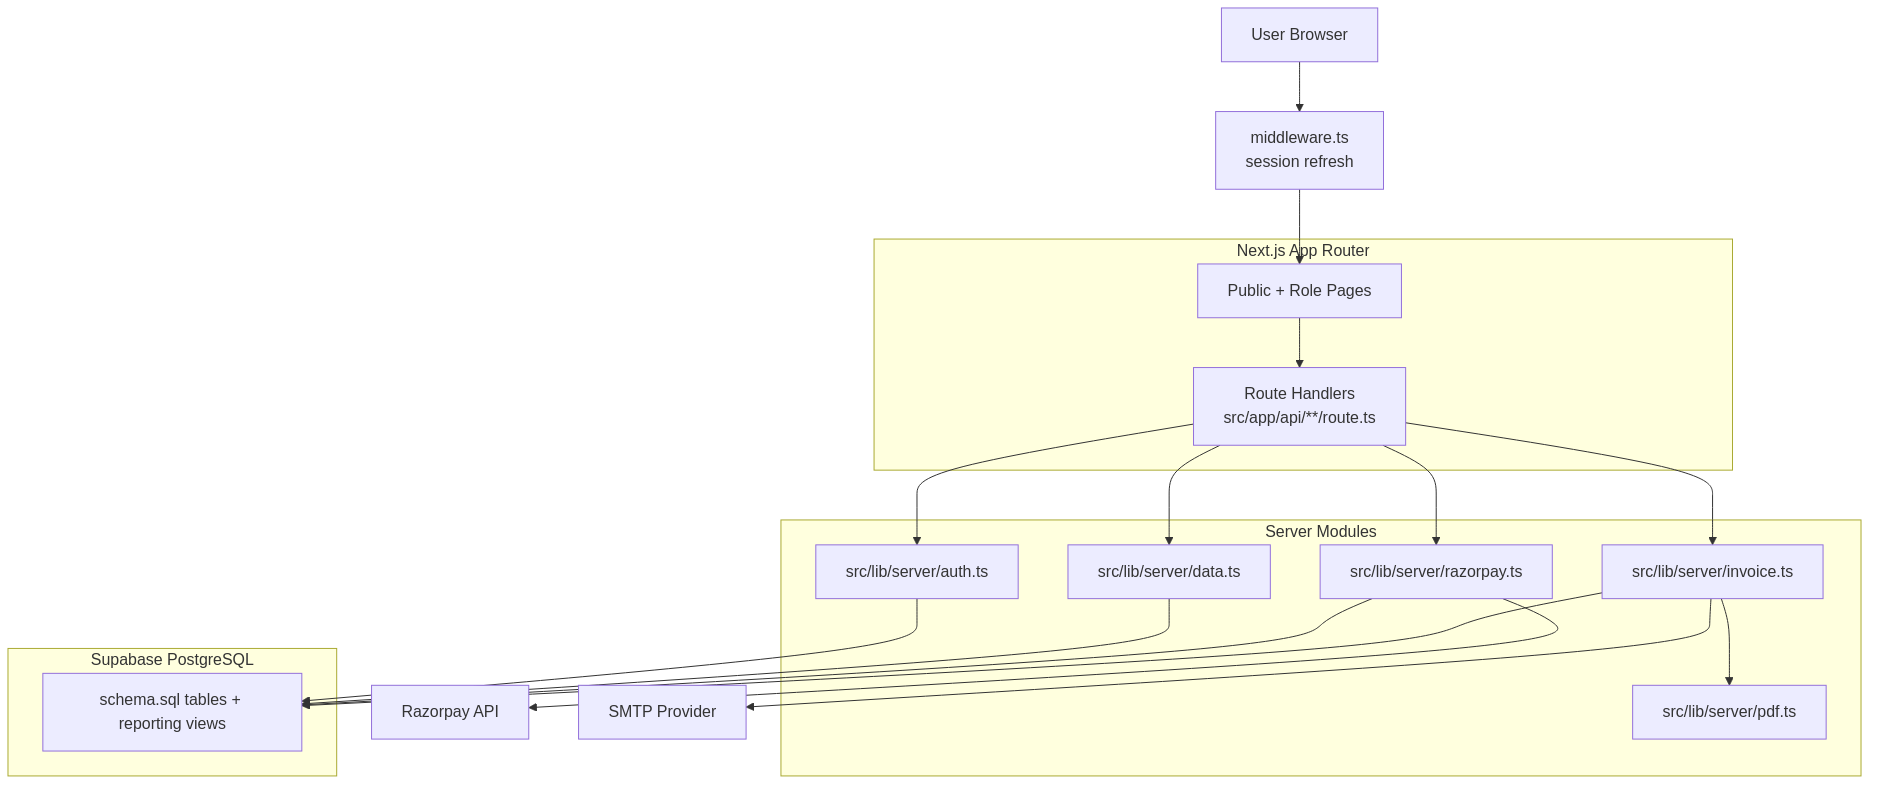
\includegraphics[width=\textwidth,height=0.75\textheight,keepaspectratio]{assets/system_architecture.png}
	\caption{Figure 5.1: System Architecture Diagram (implemented components).}
\end{figure}

\begin{figure}[H]
	\centering
	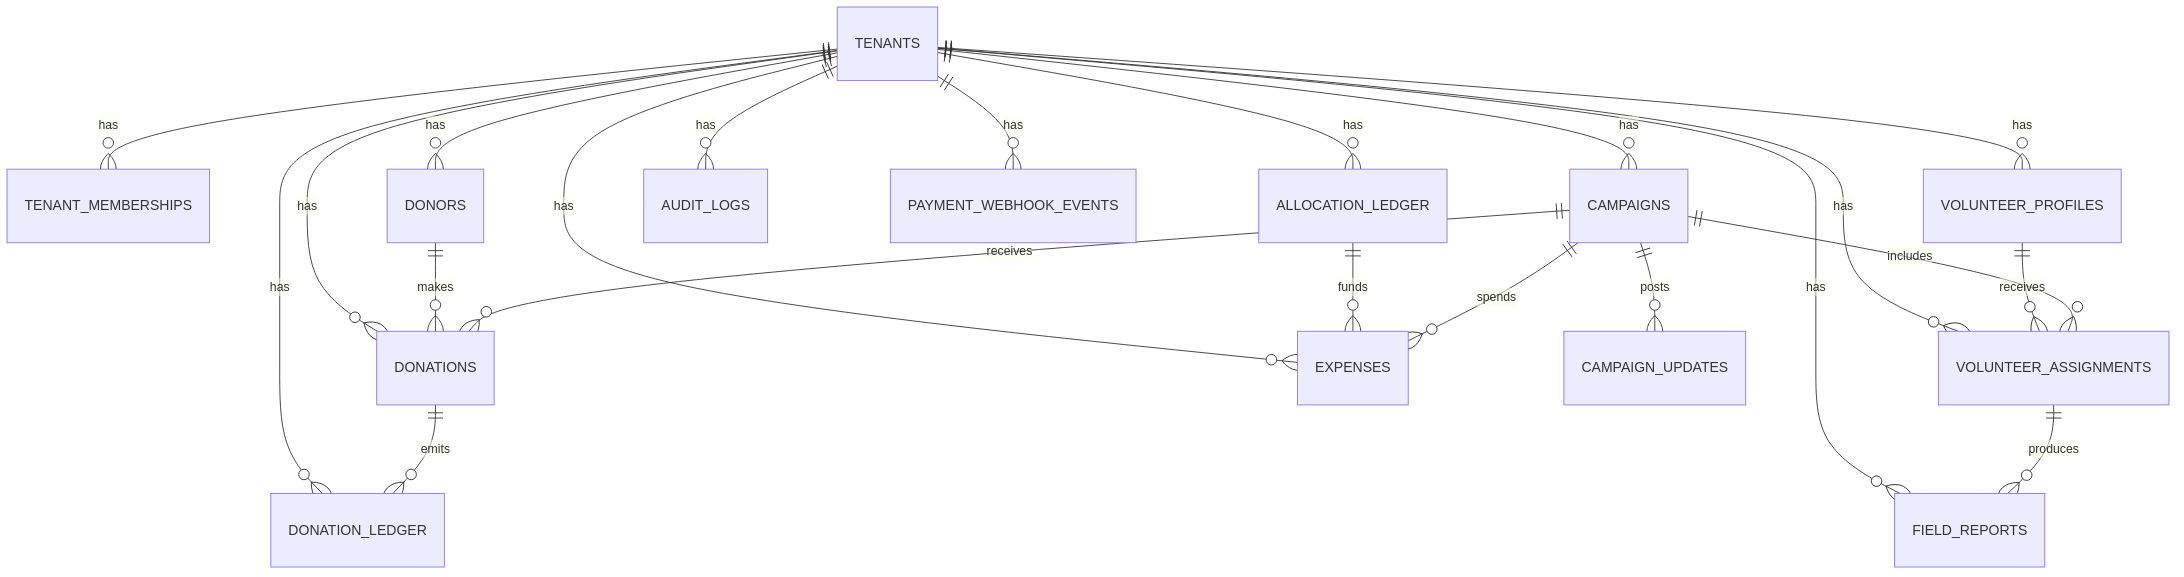
\includegraphics[width=\textwidth,height=0.75\textheight,keepaspectratio]{assets/er_diagram.png}
	\caption{Figure 5.2: Entity-Relationship Diagram based on Supabase schema.}
\end{figure}

\begin{figure}[H]
	\centering
	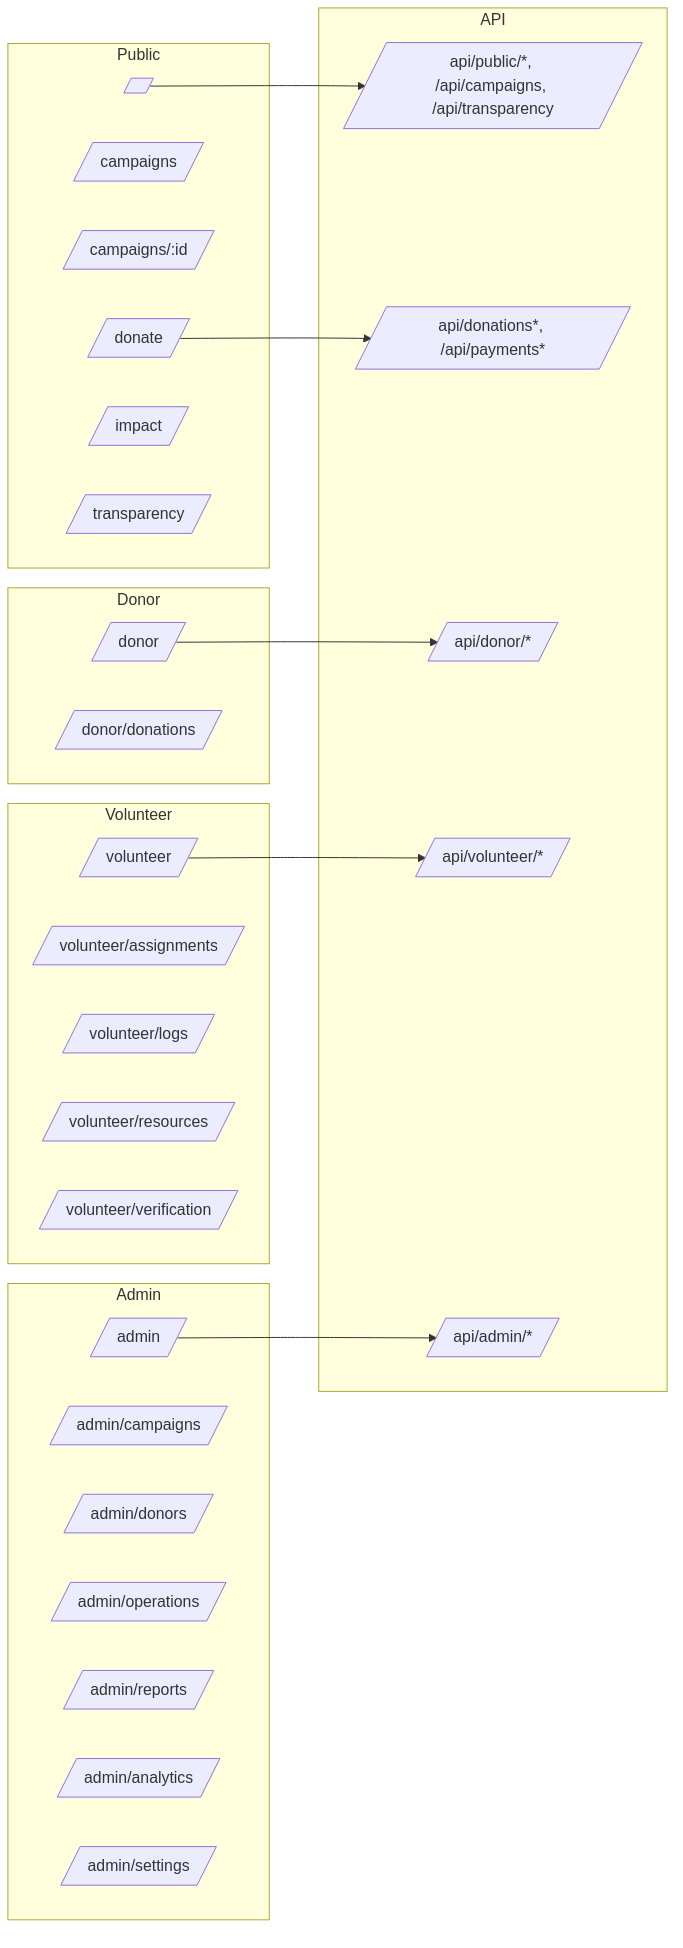
\includegraphics[width=\textwidth,height=0.75\textheight,keepaspectratio]{assets/route_map.png}
	\caption{Figure 5.3: Route and module interaction view from current app routes and APIs.}
\end{figure}

\begin{figure}[H]
	\centering
	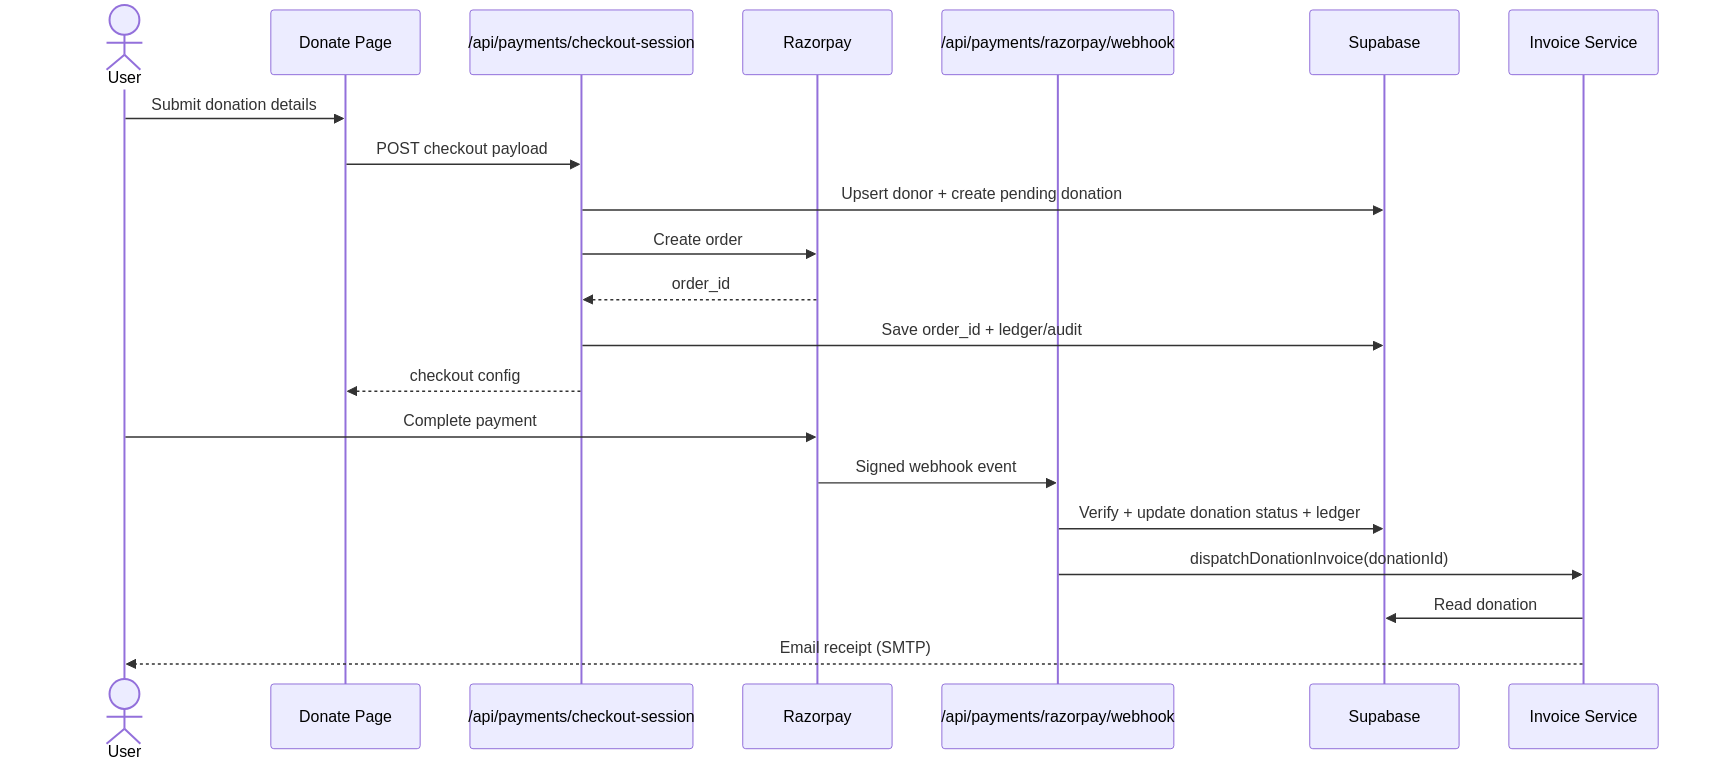
\includegraphics[width=\textwidth,height=0.75\textheight,keepaspectratio]{assets/donation_sequence.png}
	\caption{Figure 5.4: Sequence Diagram --- Donation Processing Flow.}
\end{figure}

\begin{figure}[H]
	\centering
	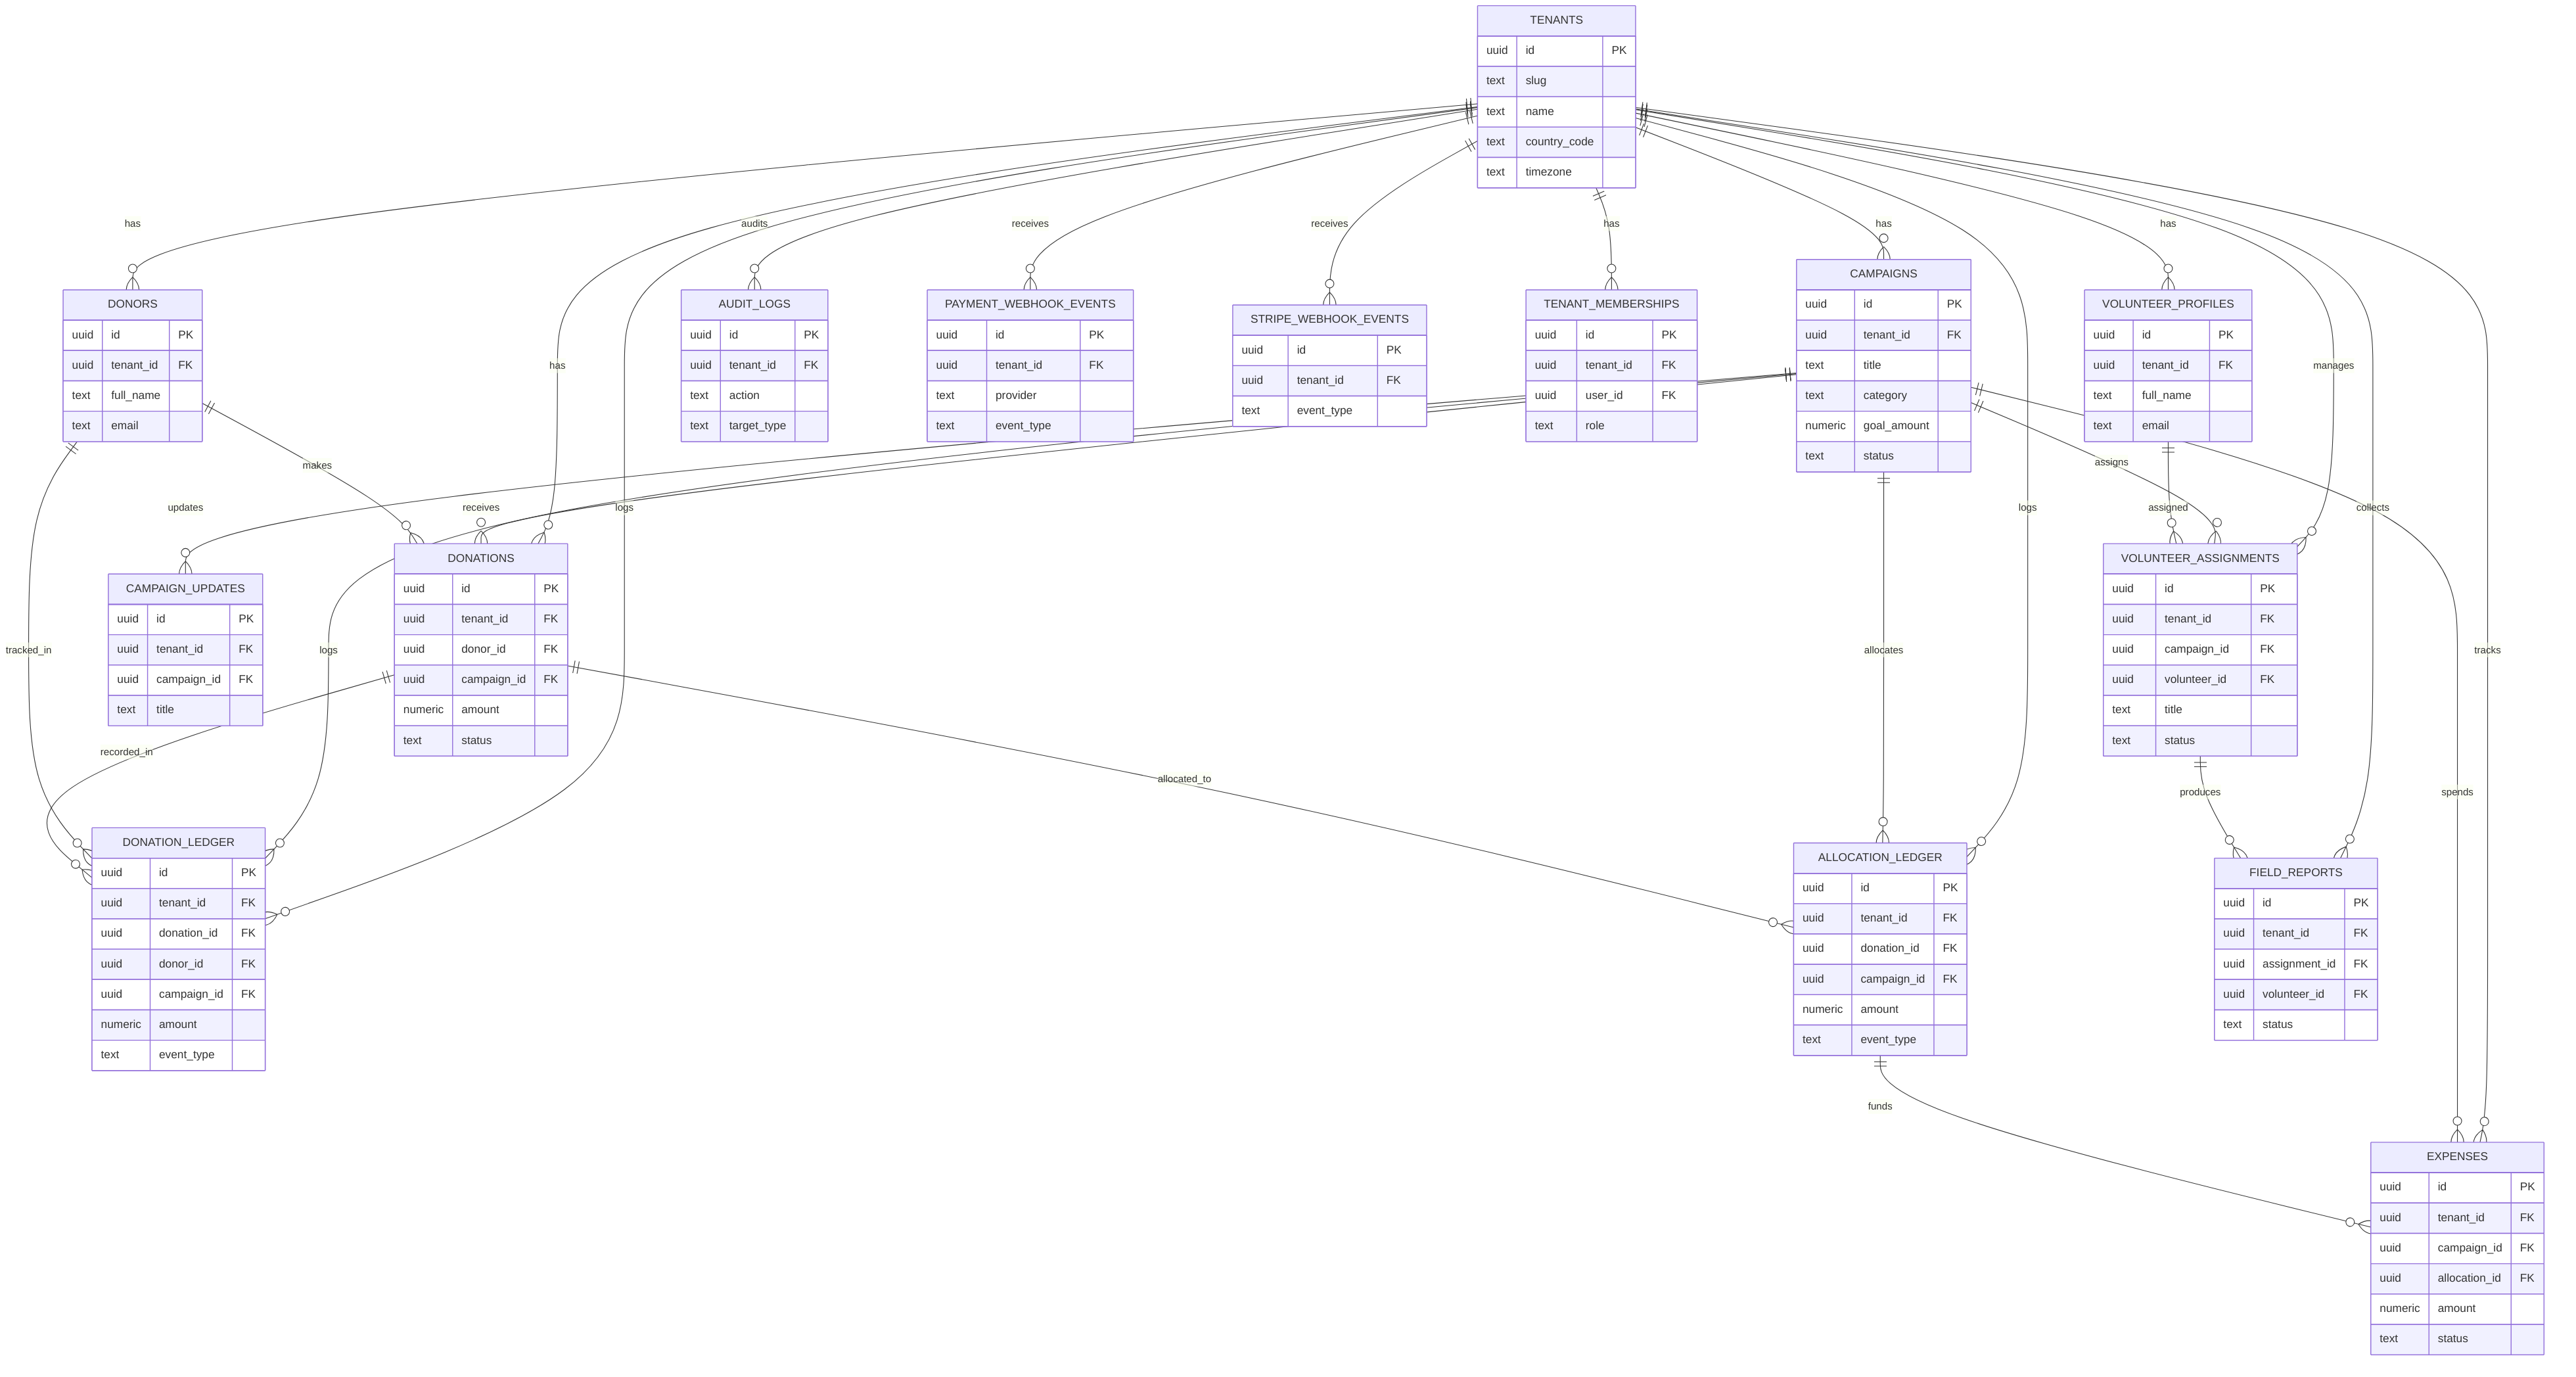
\includegraphics[width=\textwidth,height=0.75\textheight,keepaspectratio]{assets/schema.png}
	\caption{Figure 5.5: Database Schema Diagram.}
\end{figure}

\newpage
\section{CHAPTER 6\\METHODOLOGY}
The development of ImpactLedger followed an iterative methodology with repeated implementation and validation cycles. Each cycle involved planning, module development, integration checks, and review of observed behavior in API and UI surfaces. This approach was suitable for a community-engaged project where requirements were refined progressively through partner interaction and code-level verification.

The technology stack was selected based on maintainability, ecosystem maturity, and fit to project requirements. The frontend was implemented using React with Next.js. The backend behavior is implemented through Next.js route handlers and server modules. Data persistence uses Supabase PostgreSQL with tenant-scoped schema definitions and reporting views. Payments are integrated through Razorpay APIs and signed webhook processing.

\begin{figure}[H]
	\centering
	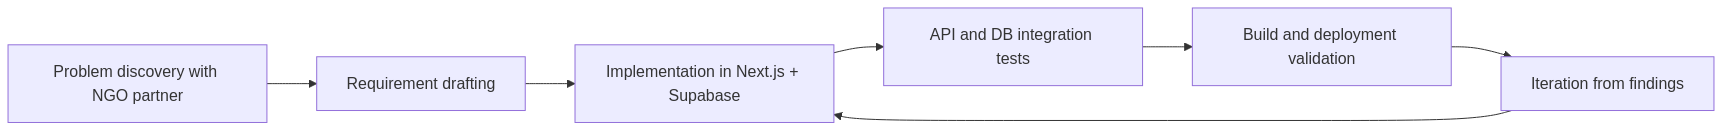
\includegraphics[width=\textwidth,height=0.7\textheight,keepaspectratio]{assets/methodology_workflow.png}
	\caption{Figure 6.1: Development methodology workflow used for implementation and verification.}
\end{figure}

\begin{figure}[H]
	\centering
	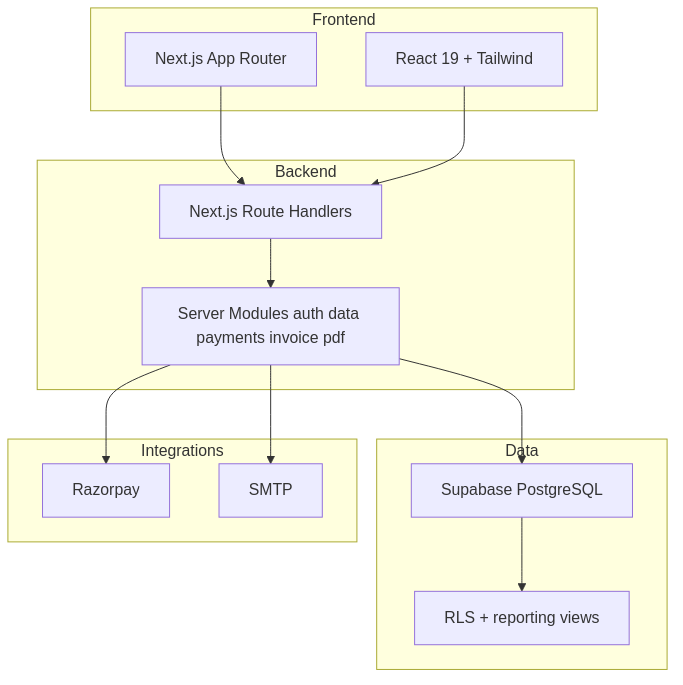
\includegraphics[width=\textwidth,height=0.7\textheight,keepaspectratio]{assets/stack_overview.png}
	\caption{Figure 6.2: Technology stack overview from repository dependencies and modules.}
\end{figure}

\newpage
\section{CHAPTER 7\\IMPLEMENTATION}
The implementation of ImpactLedger is organized into three primary modules: frontend, backend, and database integration.

The frontend module, developed using React and Next.js, includes login and signup interfaces, donor/volunteer/admin dashboards, campaign browsing and detail pages, donation pages, transparency views, and role-specific management screens.

The backend module is implemented through Next.js route handlers. It exposes API endpoints for authentication support, campaign retrieval, donation lifecycle handling, payment verification, webhook processing, reporting, analytics, and role-specific dashboards.

The database module uses Supabase PostgreSQL schema objects and views. Relationships are represented through foreign keys and tenant-scoped constraints. Event persistence is handled through ledger and webhook event tables to support auditing.

The deployed application is accessible at \url{https://impact-ledger-cep.vercel.app/} and source code is available at \url{https://github.com/SaptanshuWanjari/ImpactLedger}.

Implementation mapping:
\begin{itemize}
	\item Frontend pages under \code{src/app/**/page.tsx}
	\item Backend route handlers under \code{src/app/api/**/route.ts}
	\item Server modules under \code{src/lib/server/*}
	\item Supabase schema and migrations under \code{supabase/}
\end{itemize}

Razorpay checkout, webhook verification, invoice dispatch, and ledger persistence are implemented and connected through these modules.

\newpage
\subsection{Table 7.1: Screenshot Placement Guide for Chapter 7}
\begin{longtable}{p{0.12\textwidth}p{0.24\textwidth}p{0.35\textwidth}p{0.22\textwidth}}
	\toprule
	Figure No. & Screen / View             & Capture Instructions                                      & Placement in Report                     \\
	\midrule
	7.1        & Homepage / Landing Page   & Capture above-the-fold view of the deployed landing page. & After chapter introduction              \\
	7.2        & User Registration / Login & Capture login and signup forms with key fields visible.   & After authentication module description \\
	7.3        & Admin Dashboard           & Capture summary cards and at least one chart.             & After dashboard module description      \\
	7.4        & Campaign Creation Form    & Capture form with title/category/date/description fields. & After campaign management description   \\
	7.5        & Project/Campaign Listing  & Capture list view with status indicators.                 & After listing functionality description \\
	7.6        & Activity Log Interface    & Capture volunteer/admin logging interface.                & After activity logging description      \\
	7.7        & Donation Recording Page   & Capture donation entry or donation summary view.          & After donation recording description    \\
	7.8        & Impact Visualization      & Capture charts with labeled axes.                         & After impact dashboard description      \\
	\bottomrule
\end{longtable}

\newpage
\section{CHAPTER 8\\RESULTS AND IMPACT}
The ImpactLedger platform demonstrates working behavior across core functional areas in repository-backed validation paths. API routes for public, donor, volunteer, and admin surfaces are implemented and exercised in integration tests. The frontend renders role-specific and public pages, and data records can be created and retrieved through server handlers.

Code-backed validation signals:
\begin{itemize}
	\item build passes using \code{npm run build};
	\item integration tests pass (11/11) in \code{tests/api.integration.test.mjs};
	\item payment event lifecycle is captured through \code{donation_ledger} and \code{payment_webhook_events};
	\item transparency and overview endpoints provide public reporting views.
\end{itemize}

\subsection{Table 8.1: Before vs After Comparison --- ImpactLedger Implementation}
\begin{longtable}{p{0.25\textwidth}p{0.33\textwidth}p{0.33\textwidth}}
	\toprule
	Parameter             & Before digitization (community workflow)   & With ImpactLedger implementation                  \\
	\midrule
	Record keeping        & Fragmented manual records and spreadsheets & Structured tenant-scoped database records         \\
	Donation tracking     & Limited event traceability                 & Checkout + webhook + ledger event chain           \\
	Role visibility       & Ad-hoc information sharing                 & Role-based dashboard and API access               \\
	Transparency          & Delayed manual reports                     & Public overview and transparency ledger endpoints \\
	Operational reporting & Manual consolidation effort                & Query-backed dashboards and reporting APIs        \\
	\bottomrule
\end{longtable}

\newpage
\subsection{Table 8.2: System Performance Metrics --- ImpactLedger}
\begin{longtable}{p{0.28\textwidth}p{0.18\textwidth}p{0.28\textwidth}p{0.16\textwidth}}
	\toprule
	Metric                      & Target                      & Observed Result                       & Status \\
	\midrule
	Build integrity             & Successful production build & \code{npm run build} passed           & Pass   \\
	API integration coverage    & Core route validation       & 11/11 integration tests passed        & Pass   \\
	Payment reconciliation path & Signed webhook handling     & Implemented and persisted             & Pass   \\
	Audit trail persistence     & Event-level storage         & Donation/webhook/audit tables present & Pass   \\
	\bottomrule
\end{longtable}

\section{CHAPTER 9\\DISCUSSION}
The revised report preserves template structure while replacing outdated technical assumptions with code-backed descriptions. On the technical side, integration across dynamic dashboards, role-specific APIs, and payment reconciliation required careful server-module coordination. Ensuring consistent behavior across donor, volunteer, and admin paths required robust tenant and role handling.

The system has limitations in the current implementation phase. Runtime behavior depends on external services and correct environment configuration (Supabase, Razorpay, SMTP). Some repository validation tooling currently has baseline issues (for example ESLint configuration errors) that are separate from application runtime correctness.

From a project management perspective, aligning documentation with actual implemented behavior required careful claim-by-claim verification against source code and schema artifacts.

\section{CHAPTER 10\\CONCLUSION AND FUTURE SCOPE}
ImpactLedger currently provides a full-stack implementation for NGO campaign transparency, role-based operations, and donation reconciliation. The revised report now aligns technical claims with what is actually implemented in repository code, schema, APIs, and build/test evidence.

Future scope can include richer notification channels, enhanced analytics, deeper automation for reporting exports, and broader mobile-first optimization, provided these are implemented and verified before being described as completed features.

\section{QUICK REFERENCE: ALL FIGURES AND TABLES}
\begin{longtable}{p{0.18\textwidth}p{0.2\textwidth}p{0.52\textwidth}}
	\toprule
	Figure / Table No. & Chapter   & Description                                   \\
	\midrule
	Table 4.1          & Chapter 4 & Functional Requirements of ImpactLedger       \\
	Table 4.2          & Chapter 4 & Non-Functional Requirements of ImpactLedger   \\
	Table 4.3          & Chapter 4 & Hardware and Software Requirements            \\
	Figure 5.1         & Chapter 5 & System Architecture Diagram                   \\
	Figure 5.2         & Chapter 5 & Entity-Relationship Diagram                   \\
	Figure 5.3         & Chapter 5 & Route and Module Interaction View             \\
	Figure 5.4         & Chapter 5 & Sequence Diagram --- Donation Processing Flow \\
	Figure 6.1         & Chapter 6 & Development Methodology Workflow              \\
	Figure 6.2         & Chapter 6 & Technology Stack Overview                     \\
	Table 7.1          & Chapter 7 & Screenshot Placement Guide                    \\
	Table 8.1          & Chapter 8 & Before vs After Comparison                    \\
	Table 8.2          & Chapter 8 & System Performance Metrics                    \\
	\bottomrule
\end{longtable}

\section{REFERENCES}
GitHub Repository: \url{https://github.com/SaptanshuWanjari/ImpactLedger}\\
Deployed Application: \url{https://impact-ledger-cep.vercel.app/}\\
Next.js Documentation: \url{https://nextjs.org/docs}\\
Supabase Documentation: \url{https://supabase.com/docs}\\
Razorpay API Documentation: \url{https://razorpay.com/docs/api/}\\
React Documentation: \url{https://react.dev/}

\newpage
\section{APPENDICES}
Appendix A: Screenshots of the ImpactLedger web application

\begin{figure}[H]
	\centering
	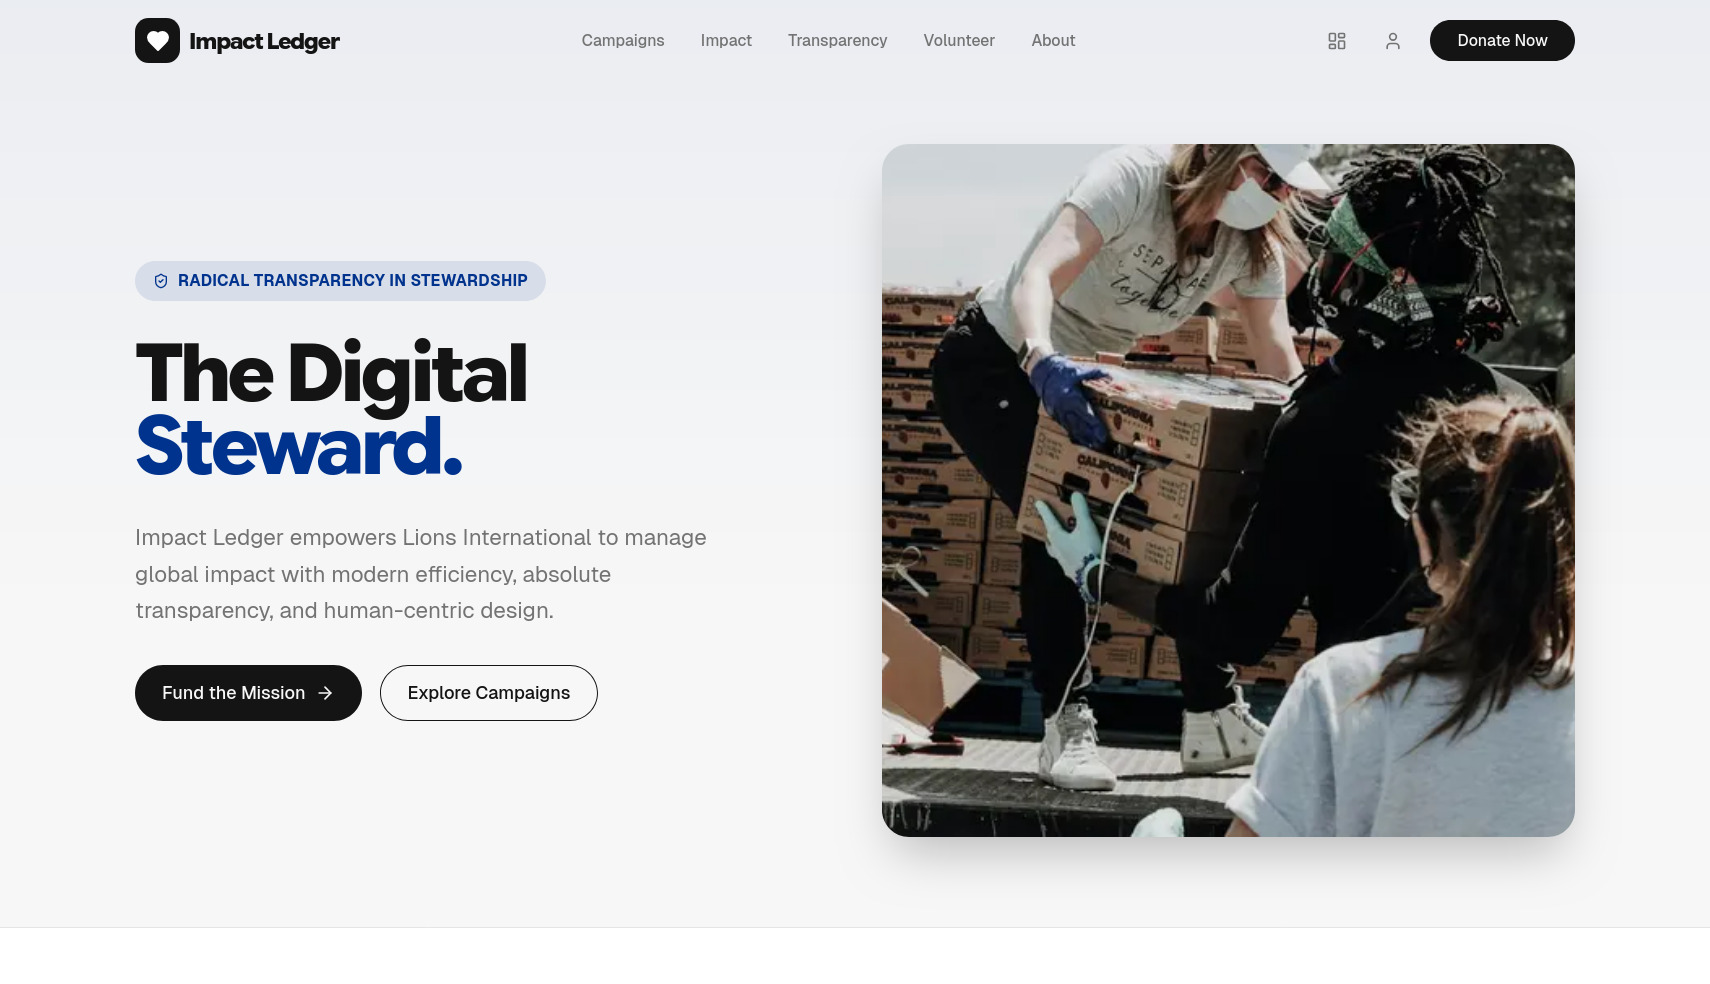
\includegraphics[width=\textwidth,keepaspectratio]{landingpage.png}
	\caption{Homepage / Landing Page}
\end{figure}

\begin{figure}[H]
	\centering
	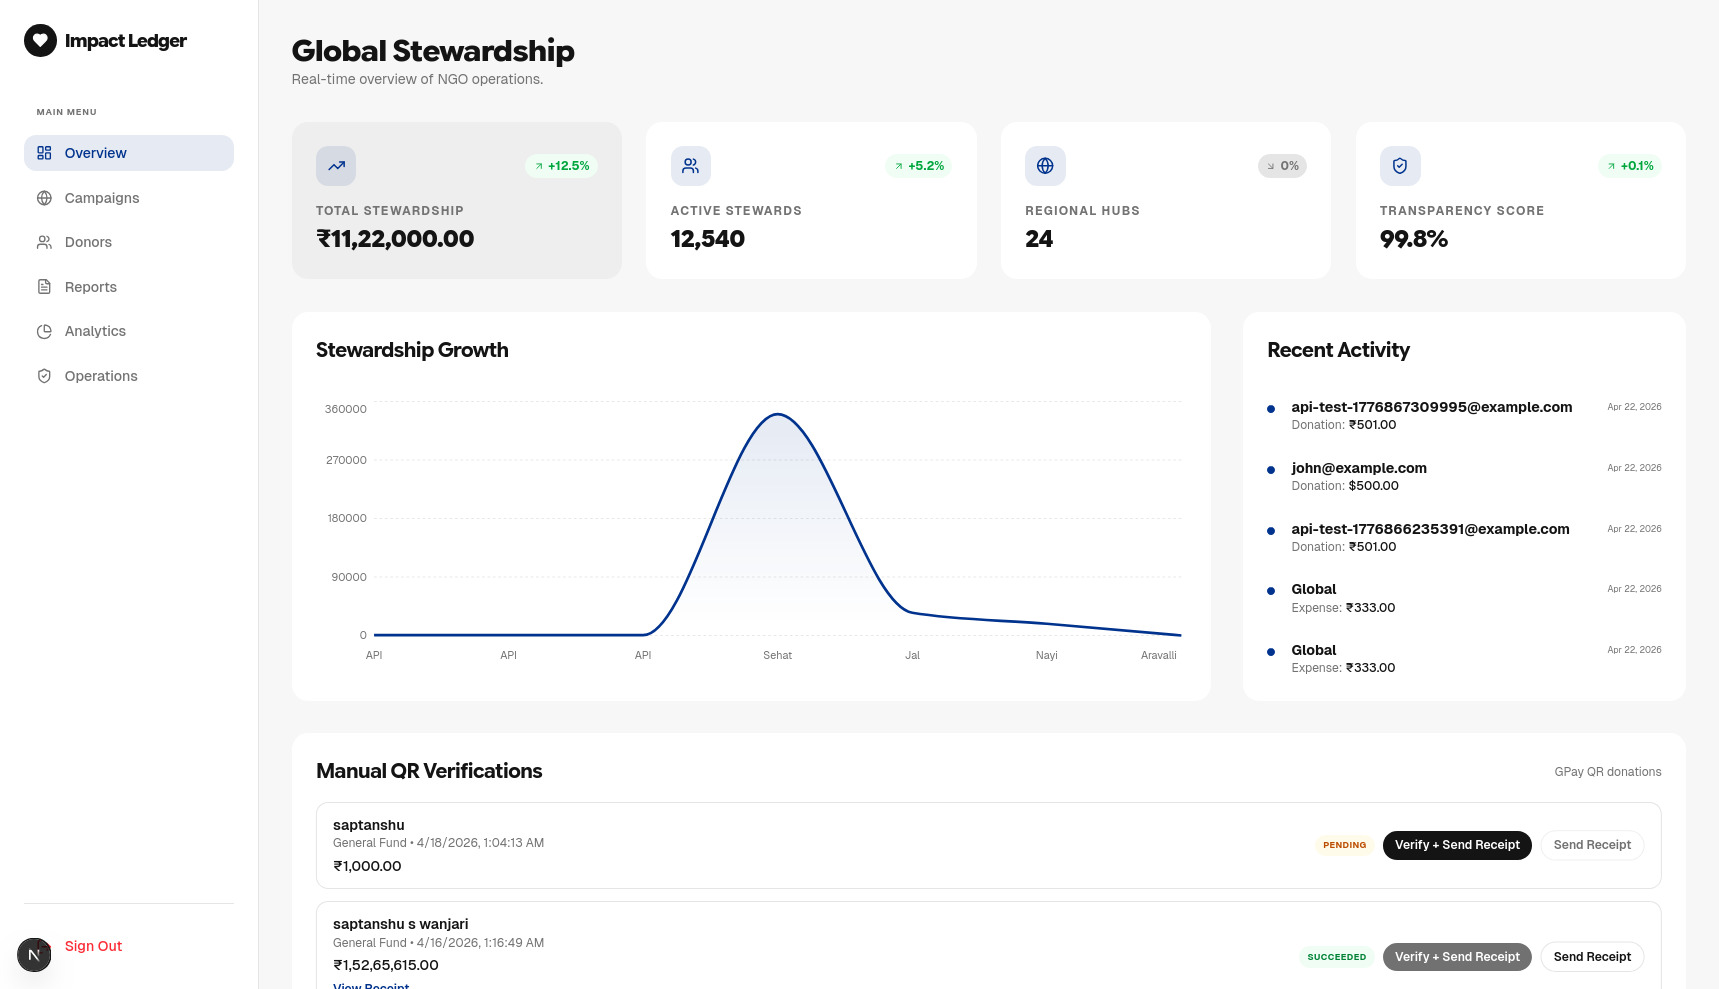
\includegraphics[width=\textwidth,keepaspectratio]{admindashboard.png}
	\caption{Admin Dashboard}
\end{figure}

\begin{figure}[H]
	\centering
	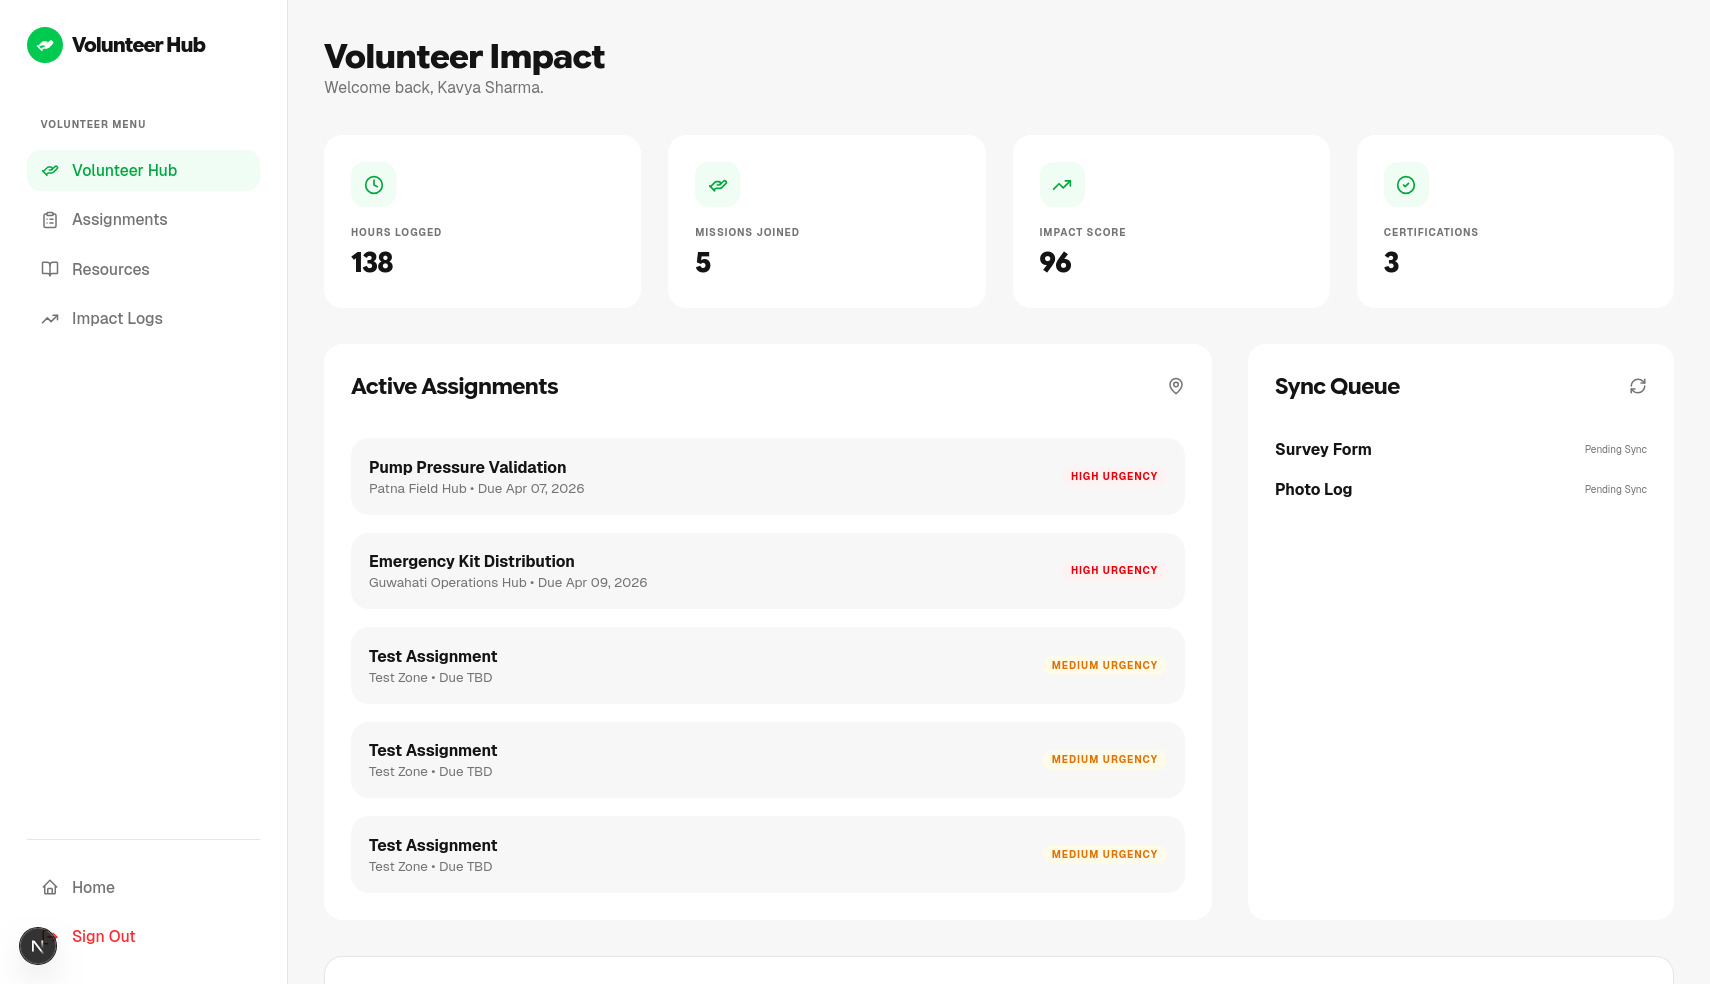
\includegraphics[width=\textwidth,keepaspectratio]{volunteerpage.png}
	\caption{Volunteer Assignments Page}
\end{figure}

\begin{figure}[H]
	\centering
	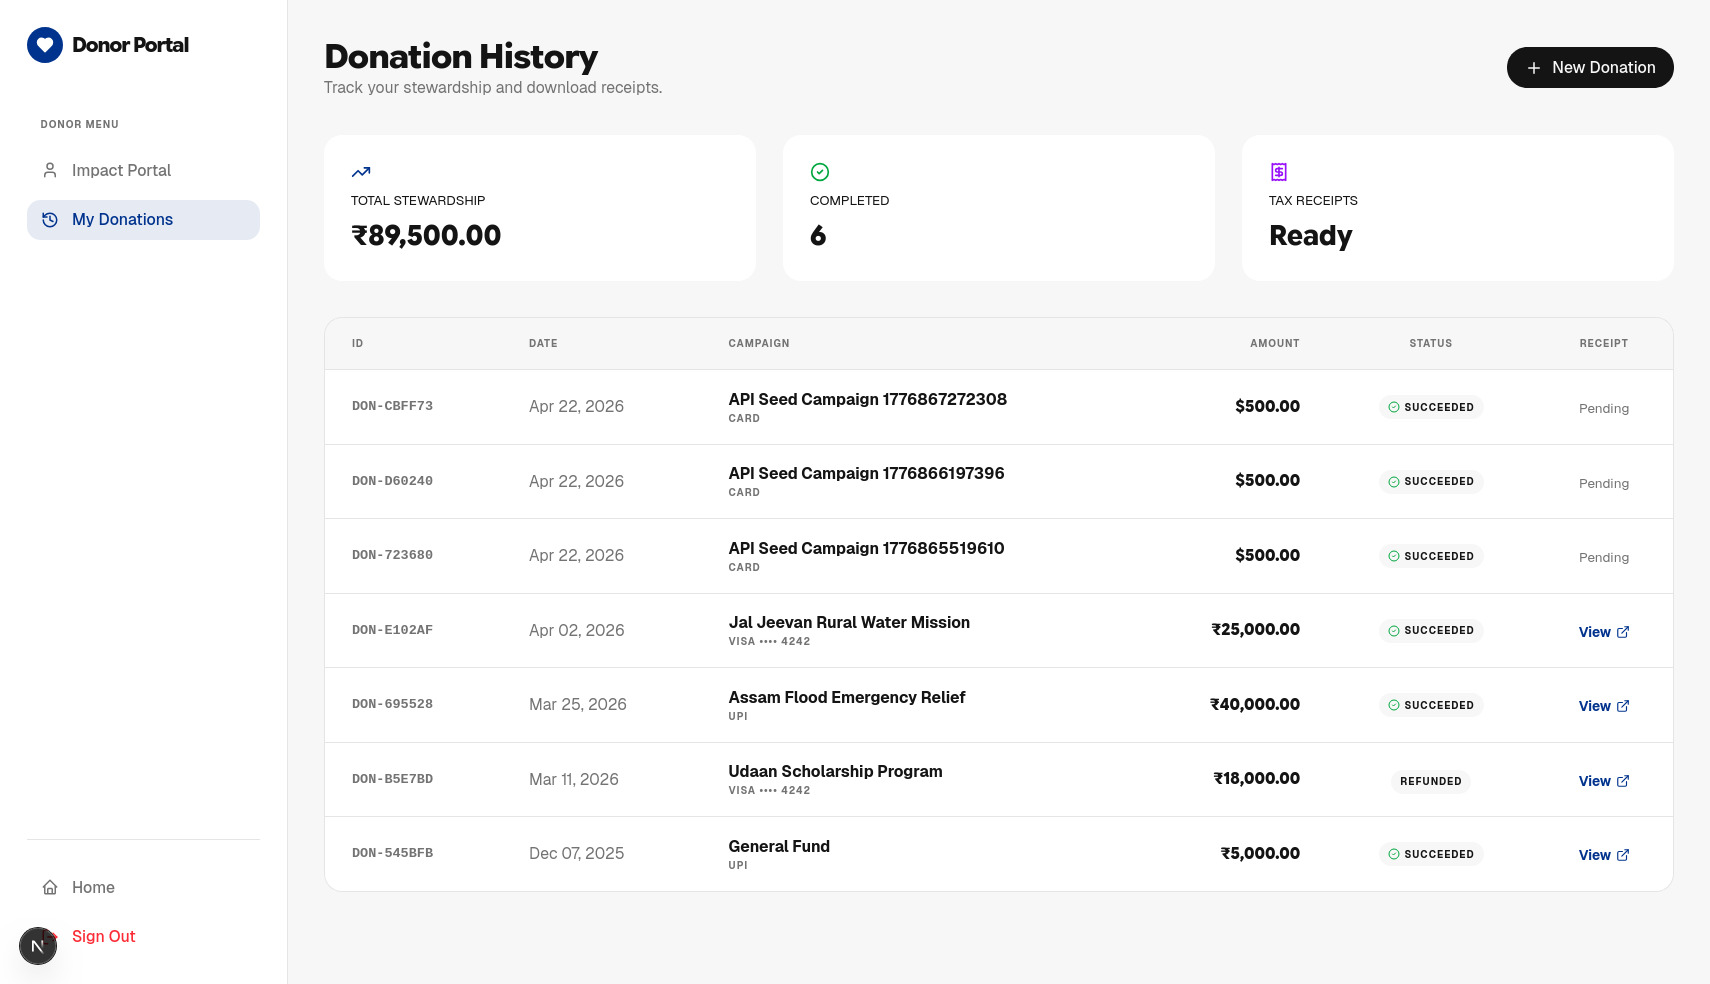
\includegraphics[width=\textwidth,keepaspectratio]{donationpage.png}
	\caption{Donor Portal Page}
\end{figure}

\end{document}
